\paragraph{1.2.1. Extract Features Layers (Tầng trích xuất đặc trưng)}
\indent\indent Đây là tầng nhận dữ liệu đồ thị từ ba phương thức khác nhau. Kiến trúc của tầng này được minh họa tại \textbf{Hình \ref{fig:KTExtractFeaturesLayers}}, bao gồm ba nhánh xử lý độc lập:\vspace{-0.1cm}
\begin{itemize}[label={--}, itemsep=1pt]
    \item Extract Image Features Layer: Sử dụng backbone CNN đã được đóng băng tham số và BatchNorm để trích xuất đặc trưng hình ảnh. Đầu ra từ backbone được đưa qua một tầng Linear để chiếu về chiều không gian vector mong muốn (448 chiều).
    \item Extract Text Features Layer: Kết hợp vector embedding của từ (Word) và câu (Sentence).
    \item Extract Audio Features Layer: Xử lý đặc trưng MFCC kết hợp với các giá trị Delta và Delta-Delta.
\end{itemize}

\begin{figure}[H]
    \centering
    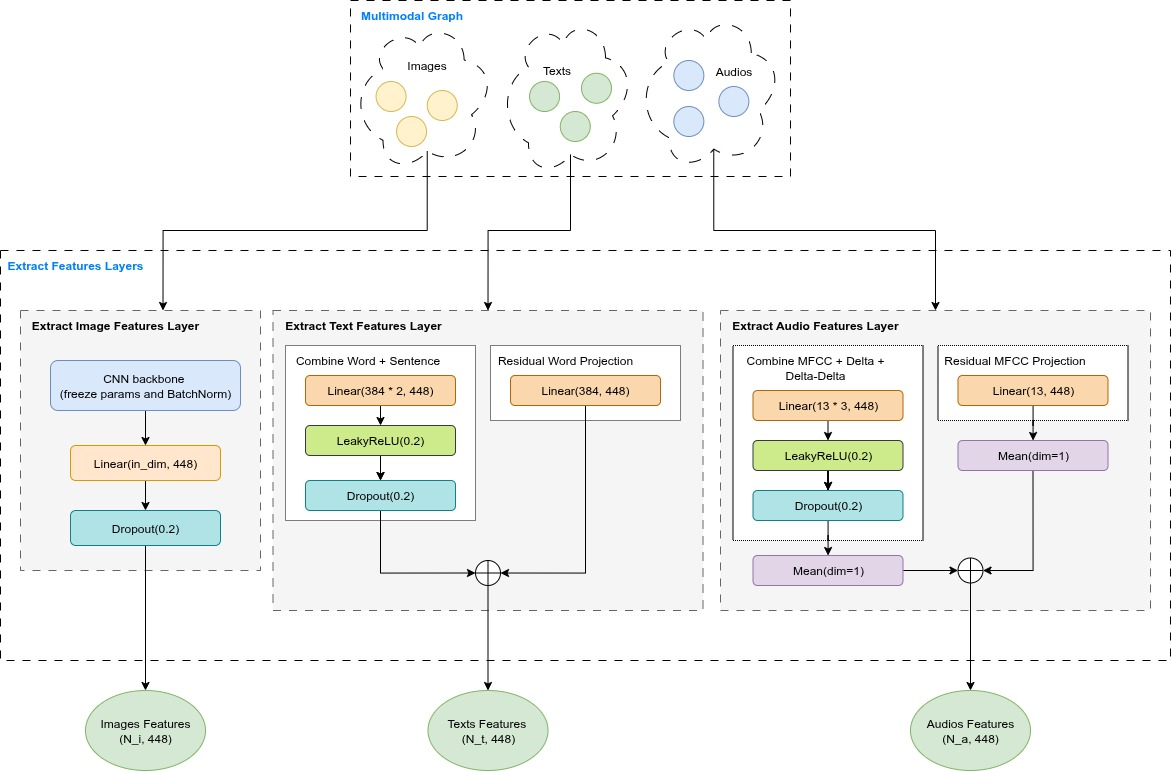
\includegraphics[width=\linewidth]{images/part-02/chap-02/sec-01/ExtractFeaturesLayers.jpg}
    \vspace{0.3cm}
    \caption{Kiến trúc chi tiết của Extract Features Layers}
    \label{fig:KTExtractFeaturesLayers}
\end{figure}

Đối với nhánh đặc trưng hình ảnh, do backbone đã cung cấp các vector đặc trưng giàu thông tin ngữ nghĩa, mô hình chỉ áp dụng phép chiếu tuyến tính đơn giản. Ngược lại, đối với văn bản và âm thanh, mô hình áp dụng cơ chế Residual Connection bằng cách cộng vector đặc trưng gốc (đã được chiếu về cùng chiều) vào đầu ra cuối cùng của nhánh. Kỹ thuật này giúp giải quyết vấn đề biến mất đạo hàm khi huấn luyện mạng sâu, đồng thời bảo toàn thông tin gốc quan trọng trước các phép biến đổi phi tuyến có thể gây mất mát thông tin đặc trưng \cite{he2015deepresiduallearningimage}.